\documentclass[12pt]{article}

% --------------------
% Basic Packages
% --------------------
\usepackage[a4paper,margin=1in]{geometry}
\usepackage{setspace}
\usepackage{graphicx}
\usepackage{amsmath}
\usepackage{amssymb}
\usepackage{booktabs}
\usepackage{microtype}
\emergencystretch=1em
\onehalfspacing

% --------------------
% Title and Author
% --------------------
\title{Energy-Aware Routing Protocols for Smart Agriculture and Precision Farming}
\author{Pranav Sista}
\date{}

\begin{document}

\maketitle

\section{Introduction}

The integration of wireless sensor networks into modern agricultural practices has revolutionized the way farmers monitor and manage crops, livestock, and environmental conditions in precision farming systems. Precision agriculture relies on real-time data collection from distributed sensor nodes to optimize resource utilization, minimize waste, and enhance yield quality while addressing the challenges of climate variability and resource scarcity. However, the deployment of these networks in remote and expansive farmlands introduces significant constraints, particularly in terms of energy consumption, as sensor nodes are typically battery-powered and must operate autonomously for extended periods without frequent maintenance. Energy-aware routing protocols emerge as a critical solution to extend network lifetime, ensure reliable data transmission, and support sustainable operations in smart agriculture environments.

In the context of smart agriculture, wireless sensor networks facilitate applications such as soil moisture monitoring, automated irrigation scheduling, pest detection, and microclimate assessment, all of which demand continuous data flow from field-deployed nodes to a central sink or base station. Traditional routing approaches often lead to rapid energy depletion due to unbalanced load distribution and inefficient data aggregation, resulting in network partitioning and loss of critical agricultural insights. This paper examines energy-aware routing protocols tailored for such scenarios, emphasizing their role in balancing energy efficiency with the unique demands of precision farming, including variable terrain, heterogeneous sensor types, and the need for low-latency decision-making in dynamic environmental conditions. The discussion incorporates detailed mathematical formulations of energy consumption to provide a rigorous quantitative foundation for protocol evaluation.

The primary objective of this analysis is to provide a thorough evaluation of established and emerging protocols that incorporate energy optimization mechanisms, while highlighting their applicability to real-world agricultural deployments. By exploring foundational concepts, core methodologies, comparative performance metrics, practical implementations, associated challenges, and prospective advancements, this study contributes to the growing body of knowledge on sustainable wireless communication in agritech. Mathematical formulations of energy consumption models are integrated to quantify protocol efficacy, supported by illustrative figures and tables that visualize key performance indicators. Through this structured investigation, the paper underscores the transformative potential of energy-aware routing in advancing precision farming toward greater ecological and economic viability.

Subsequent sections delve into the conceptual underpinnings of wireless sensor networks within agricultural frameworks, delineate specific routing approaches with emphasis on hierarchical and artificial intelligence-enhanced variants, engage in a detailed comparative analysis, present insights from field applications, address persistent challenges, outline future research trajectories, and culminate in a synthesis of findings. This comprehensive approach ensures that the analysis not only reviews existing literature but also synthesizes interdisciplinary insights from computer science, agronomy, and environmental engineering to propose actionable pathways for implementation.

\subsection{Motivation for Energy-Aware Protocols in Precision Farming}

The motivation for developing energy-aware routing protocols stems from the inherent limitations of battery-operated sensor nodes in expansive agricultural fields, where replacement or recharging is logistically challenging and costly. Precision farming demands uninterrupted monitoring over entire growing seasons, and any premature node failure can lead to gaps in data coverage that compromise yield predictions and resource management strategies. Energy-aware designs address these issues by dynamically adapting routing decisions to residual battery levels, thereby extending the overall network lifespan and reducing the environmental impact associated with frequent hardware interventions.

\subsection{Objectives of the Study}

This study aims to systematically evaluate the performance of leading energy-aware routing protocols in the specific context of smart agriculture, with a focus on quantifying improvements in network longevity and data fidelity through mathematical modeling and comparative metrics. Additionally, the research seeks to identify practical deployment strategies that align protocol capabilities with the heterogeneous requirements of different crop types and farming scales, ultimately contributing to more resilient and sustainable agritech ecosystems.

\subsection{Scope and Limitations}

The scope of this paper encompasses hierarchical, chain-based, threshold-sensitive, multipath, and artificial intelligence-augmented routing protocols, with detailed examinations of their energy consumption behaviors in simulated and real-world agricultural settings. While the analysis prioritizes wireless sensor networks operating under the first-order radio model, it acknowledges limitations such as the exclusion of advanced energy harvesting integrations that may emerge in future iterations of precision farming technologies.

\subsection{Overall Structure of the Analysis}

The structure of the paper is designed to progress logically from foundational knowledge to applied insights and forward-looking perspectives, ensuring that each section builds upon the previous to deliver a cohesive and in-depth understanding of energy-aware routing in smart agriculture.

\section{Background and Conceptual Foundations}

Wireless sensor networks form the backbone of data acquisition in precision farming, where clusters of low-power nodes equipped with sensing, processing, and communication capabilities are distributed across agricultural landscapes to capture multifaceted environmental parameters. These networks operate under stringent energy budgets, as nodes must sustain operations amid unpredictable weather patterns and soil conditions that exacerbate power drain through frequent sensing cycles and data relay tasks. The conceptual foundation rests on the principle of collaborative sensing, wherein individual nodes aggregate and forward information to minimize redundant transmissions and conserve battery resources critical for long-term field autonomy. This collaborative paradigm is essential in precision farming, where spatial correlations in soil and crop data allow for efficient in-network processing that reduces the overall communication overhead.

A foundational aspect involves understanding the energy constraints inherent to wireless sensor deployments in agriculture. Sensor nodes typically rely on limited-capacity batteries, and their energy expenditure is dominated by radio communication activities rather than sensing or computation. In precision farming, where nodes may be placed in soil or canopy environments with limited solar recharging opportunities, protocols must prioritize energy balancing to prevent premature node failures that could compromise entire monitoring zones dedicated to crop health assessment or water management. The first-order radio model serves as a cornerstone for these analyses, providing quantifiable expressions for energy dissipation that guide protocol design.

The evolution of routing strategies in wireless sensor networks draws from broader ad hoc networking paradigms but adapts specifically to the data-centric and location-aware requirements of agricultural monitoring. Early models emphasized direct transmission to a base station, which proved inefficient for large-scale farms due to disproportionate energy use by distant nodes. This limitation prompted the development of multi-hop and hierarchical schemes that distribute load more equitably, incorporating factors such as residual energy, proximity to the sink, and data correlation typical in soil humidity or temperature gradients across fields. These adaptations ensure that routing decisions remain aligned with the temporal and spatial dynamics of agricultural processes.

Precision farming imposes unique requirements on these networks, including scalability to cover vast hectares, robustness against node mobility induced by farm machinery, and integration with emerging technologies like unmanned aerial vehicles for hybrid data collection. Conceptual models must account for the spatial variability in agricultural fields, where sensor density varies by crop type—higher in high-value orchards compared to broad-acre cereals—and where data urgency fluctuates with seasonal events such as irrigation needs during drought periods. These foundations underscore the necessity for routing protocols that not only conserve energy but also align with the decision-support systems driving smart agriculture, ensuring that energy optimization translates directly into actionable insights for farmers.

\subsection{Architectural Components of Wireless Sensor Networks in Agriculture}

The architecture of wireless sensor networks deployed for smart agriculture typically comprises three primary layers: the sensing layer with heterogeneous nodes for parameters like soil pH, moisture, and nutrient levels; the networking layer responsible for data routing and aggregation; and the application layer interfacing with farmer dashboards or cloud-based analytics platforms. In precision farming, nodes are often organized in clusters to facilitate localized processing, reducing the volume of raw data transmitted over long distances and thereby mitigating energy overhead in expansive fields. This layered approach enables seamless integration of sensing modalities tailored to specific agronomic needs, such as integrating optical sensors for leaf health with subsurface probes for root zone analysis.

\subsection{Energy Dissipation Models in Resource-Constrained Environments}

Energy models provide the mathematical bedrock for evaluating routing efficiency. The first-order radio model, widely adopted in wireless sensor network literature, quantifies transmission and reception costs as follows. Let \( k \) represent the packet size in bits and \( d \) the transmission distance. The energy consumed for transmitting a packet is given by

\begin{equation}
E_{Tx}(k, d) = E_{elec} \cdot k + \epsilon_{amp} \cdot k \cdot d^{2}
\end{equation}

where \( E_{elec} \) denotes the electronics energy per bit, typically 50 nJ/bit, and \( \epsilon_{amp} \) is the amplifier energy, often 100 pJ/bit/m\textsuperscript{2} for free-space propagation. Reception energy is modeled as

\begin{equation}
E_{Rx}(k) = E_{elec} \cdot k
\end{equation}

These equations illustrate how distance-squared dependency amplifies energy costs in direct long-range communications, a critical consideration for agricultural deployments spanning hundreds of meters between field edges and base stations. Extensions to this model incorporate amplifier factors for multipath fading in foliage-dense environments, expressed as \( \epsilon_{amp} \cdot k \cdot d^{4} \) when \( d \) exceeds a crossover distance threshold.

\subsection{Interdisciplinary Intersections in Precision Farming Networks}

Precision farming bridges agronomic principles with communication theory, where routing decisions must incorporate crop-specific phenological stages that influence data generation rates. For instance, during peak growth phases, higher sampling frequencies necessitate protocols that dynamically adjust cluster formations to balance energy load without sacrificing temporal resolution in pest or disease monitoring. This intersection fosters innovations that leverage agronomic knowledge to inform network topology optimizations, such as placing higher-energy cluster heads in zones with elevated data variability.

\subsection{Historical Development of WSN Routing in Agricultural Contexts}

The historical development of wireless sensor network routing for agriculture traces back to early deployments in the early 2000s, where basic flooding mechanisms gave way to energy-conscious designs amid growing concerns over battery longevity in remote field trials. Pioneering works established benchmarks for energy efficiency that continue to influence contemporary protocols, particularly as precision farming scaled from experimental plots to commercial operations spanning thousands of hectares.

\section{Core Concepts and Approaches}

Energy-aware routing protocols in wireless sensor networks for smart agriculture build upon hierarchical, chain-based, threshold-sensitive, and multipath strategies, each augmented by artificial intelligence techniques to address the dynamic energy profiles of field environments. These approaches prioritize residual energy awareness, data aggregation, and adaptive path selection to prolong network operational lifespan while maintaining the fidelity of agricultural data streams essential for precision interventions. Detailed examinations of these protocols reveal their underlying mechanisms and mathematical optimizations tailored to the variable conditions encountered in crop monitoring.

Hierarchical protocols such as the Low Energy Adaptive Clustering Hierarchy (LEACH) exemplify foundational concepts by electing cluster heads probabilistically based on energy levels, enabling localized data fusion before transmission to the sink. In agricultural settings, LEACH reduces overall energy expenditure by confining intra-cluster communications to short ranges, which is particularly advantageous in uniform crop fields where soil moisture data exhibits high spatial correlation. The protocol operates in rounds, with setup and steady-state phases ensuring even distribution of the cluster head role to prevent hotspot formation around high-traffic nodes monitoring irrigation zones. The probability of a node becoming a cluster head in round \( r \) is given by

\begin{equation}
T(n) = \frac{p}{1 - p \cdot (r \mod \frac{1}{p})}
\end{equation}

for nodes that have not served as cluster heads in the recent cycle, where \( p \) is the desired percentage of cluster heads.

Chain-based methodologies, exemplified by the Power-Efficient Gathering in Sensor Information Systems (PEGASIS), construct a single linear chain among nodes, with data propagating hop-by-hop toward a designated leader that communicates with the base station. This eliminates the overhead of repeated cluster formations inherent in LEACH, making PEGASIS suitable for linear agricultural layouts such as vineyard rows or contour-planted fields, where energy savings accrue from minimized long-distance transmissions and progressive data aggregation along the chain. Energy calculations in PEGASIS focus on nearest-neighbor distances to minimize cumulative \( E_{Tx} \) along the chain path.

Threshold-sensitive protocols like the Threshold Sensitive Energy Efficient sensor Network (TEEN) introduce reactive behaviors, transmitting data only when sensed values exceed predefined hard or soft thresholds. In precision farming, TEEN conserves energy during stable environmental periods, such as non-drought seasons when soil parameters change gradually, by suppressing unnecessary reports while responding promptly to critical events like sudden temperature spikes indicative of frost risk in orchards. The dual-threshold mechanism directly reduces the number of transmission events, thereby lowering the aggregate energy term \( \sum E_{Tx}(k, d) \) over operational rounds.

Multipath routing complements these by establishing multiple disjoint or braided paths from sources to the sink, enhancing reliability in error-prone agricultural wireless channels affected by foliage or weather interference. By distributing traffic across paths weighted by energy metrics, multipath schemes mitigate single-point failures and balance load, proving effective in heterogeneous farms integrating both static soil sensors and mobile nodes on drones for canopy scanning. Artificial intelligence-based enhancements elevate these core approaches through predictive optimization. Machine learning models, including reinforcement learning for dynamic path selection and particle swarm optimization for cluster head election, enable protocols to anticipate energy depletion patterns based on historical agricultural data cycles. For example, genetic algorithms can evolve routing topologies that incorporate solar harvesting potential in sun-exposed fields, while neural networks refine threshold adaptations in TEEN variants for crop-specific variability.

These core concepts integrate seamlessly with energy models to derive protocol-specific consumption profiles, ensuring that mathematical predictions align with empirical performance in precision farming trials. Hybrid variants further combine elements from multiple approaches to achieve superior adaptability in complex agricultural landscapes.

\subsection{Hierarchical and Chain-Based Routing Fundamentals}

Hierarchical structures distribute responsibility to alleviate energy imbalances, with LEACH's probabilistic selection formula serving as a cornerstone for energy-aware decision-making in clustered agricultural networks. Chain-based alternatives like PEGASIS provide complementary benefits by streamlining data paths in linearly arranged sensor deployments common in row-crop farming.

\subsection{Threshold and Reactive Mechanisms}

TEEN's dual-threshold approach minimizes transmissions, directly impacting the cumulative energy term in the first-order model by reducing \( k \) instances over time in low-variability farm microclimates. This reactivity is particularly valuable in scenarios where environmental parameters exhibit sporadic fluctuations, such as during pest infestations or irrigation events.

\subsection{Artificial Intelligence Integration in Routing}

AI-driven variants employ swarm intelligence to optimize multipath selections, iteratively minimizing the global energy function derived from aggregated \( E_{Tx} \) and \( E_{Rx} \) across candidate routes. Reinforcement learning frameworks further enable protocols to learn optimal policies from real-time feedback in dynamic field conditions.

\subsection{Hybrid Protocol Architectures for Enhanced Efficiency}

Hybrid architectures merge hierarchical clustering with threshold sensitivity and multipath redundancy, creating robust frameworks that adaptively switch between modes based on residual energy and data urgency, thereby achieving balanced performance across diverse precision farming applications.

\section{Comparative Discussion}

A comparative examination of the aforementioned protocols reveals nuanced trade-offs in energy efficiency, network lifetime, and suitability for smart agriculture applications. LEACH demonstrates robust performance in dense deployments through its adaptive clustering, yet incurs setup overhead that can elevate energy use in small-scale precision plots. In contrast, PEGASIS achieves superior energy conservation in chain configurations by limiting base station interactions to a single node per round, though it risks chain breakage in mobile or fault-prone farm environments. TEEN excels in event-driven scenarios common to precision farming, such as pest outbreaks, by curtailing proactive reporting and thereby extending node longevity beyond that of continuous protocols like LEACH. Multipath routing offers enhanced fault tolerance, distributing energy loads to sustain operations during partial network degradation from agricultural machinery interference, but at the cost of increased control packet overhead compared to single-path hierarchical schemes.

When augmented with artificial intelligence, these protocols exhibit marked improvements; for instance, PSO-optimized LEACH variants select cluster heads with greater consideration for residual energy and distance to sink, yielding up to 30 percent longer lifetimes in simulated agricultural fields relative to baseline implementations. Comparative metrics, as summarized in Table~\ref{tab:comparison}, underscore these differences across key parameters including average energy consumption per round and packet delivery ratio under varying node densities typical of crop monitoring grids. The analysis further incorporates quantitative evaluations of scalability and robustness under simulated environmental perturbations representative of real farmland conditions.

The discussion highlights that no single protocol universally dominates; instead, hybrid integrations—such as AI-enhanced TEEN with multipath fallbacks—provide optimal balances for heterogeneous precision farming ecosystems, where energy awareness must coexist with requirements for real-time alerts on soil degradation or water stress. Pairwise comparisons reveal specific strengths, such as PEGASIS outperforming LEACH in linear topologies but lagging in highly dynamic settings where AI-multipath approaches excel.

\begin{table}[htbp]
\centering
\small
\caption{Comparative Performance Metrics of Energy-Aware Routing Protocols in Simulated Agricultural WSN Deployments \cite{Jawad2017}.}
\label{tab:comparison}
\begin{tabular}{lccc}
\toprule
Protocol & Avg. Energy/Round (mJ) & Lifetime (Rounds) & PDR (\%) \\
\midrule
LEACH & 45.2 & 1200 & 92 \\
PEGASIS & 28.7 & 1850 & 88 \\
TEEN & 32.1 & 1650 & 95 \\
AI-Multipath & 24.5 & 2100 & 97 \\
\bottomrule
\end{tabular}
\end{table}

This table, derived from aggregated simulation studies, illustrates the quantitative advantages of AI integration in extending operational horizons critical for seasonal crop cycles. A second comparative perspective is provided in Table~\ref{tab:scalability}, which evaluates scalability metrics across protocols under increasing node densities.

\begin{table}[htbp]
\centering
\small
\caption{Scalability Metrics for Energy-Aware Routing Protocols in Large-Scale Precision Farming Deployments \cite{Bekal2024}.}
\label{tab:scalability}
\begin{tabular}{lcc}
\toprule
Protocol & Max Nodes Supported & Energy Efficiency at Scale (\%) \\
\midrule
LEACH & 500 & 75 \\
PEGASIS & 800 & 82 \\
TEEN & 600 & 88 \\
AI-Multipath & 1200 & 94 \\
\bottomrule
\end{tabular}
\end{table}

\subsection{Pairwise Protocol Analysis}

Pairwise evaluations between LEACH and PEGASIS highlight the former's flexibility in clustered environments versus the latter's efficiency in linear arrangements, informing selection criteria based on field geometry in precision agriculture.

\subsection{Quantitative Performance Metrics}

Quantitative assessments rely on metrics derived from the energy model equations, demonstrating how AI enhancements consistently lower per-packet costs across diverse simulation scenarios representative of agricultural variability.

\subsection{Limitations and Trade-Offs in Comparative Contexts}

Limitations such as setup overhead in hierarchical protocols and vulnerability to chain disruptions in PEGASIS underscore the need for context-specific adaptations when deploying in smart farming operations.

\section{Practical Insights and Use Cases}

Practical deployments of energy-aware routing protocols in smart agriculture demonstrate tangible benefits in enhancing decision-making precision while curtailing operational costs associated with battery replacements in remote fields. In large-scale irrigation systems across arid regions, LEACH-based networks have enabled continuous soil moisture profiling, with cluster heads aggregating data to inform variable-rate watering algorithms that reduce water consumption by up to 25 percent without compromising yield. These deployments illustrate the protocols' capacity to integrate with existing farm management software, providing farmers with actionable dashboards derived from energy-optimized data streams.

Real-world use cases further include greenhouse environments where PEGASIS chains support fine-grained temperature and humidity monitoring, facilitating automated climate control that optimizes energy use in heating and ventilation systems. TEEN protocols have proven instrumental in pest management applications, triggering alerts only upon threshold breaches in insect trap sensors, thereby conserving resources in orchards while enabling timely interventions that minimize pesticide application. Multipath and AI-enhanced approaches shine in integrated farm management platforms combining ground sensors with aerial drones, where dynamic routing adapts to node failures from weather events, ensuring uninterrupted data flow for yield prediction models.

In rice paddies of South Asia, hybrid protocols have supported flood monitoring and nutrient management, extending sensor operational periods through intelligent load balancing. Similarly, in European vineyards, threshold-sensitive variants have optimized grape quality assessments by focusing transmissions on critical phenological stages. Figure~\ref{fig:wsn-ag} depicts a typical wireless sensor network topology in a precision farming field, highlighting cluster formations and data pathways optimized for energy efficiency.

\begin{figure}[htbp]
\centering
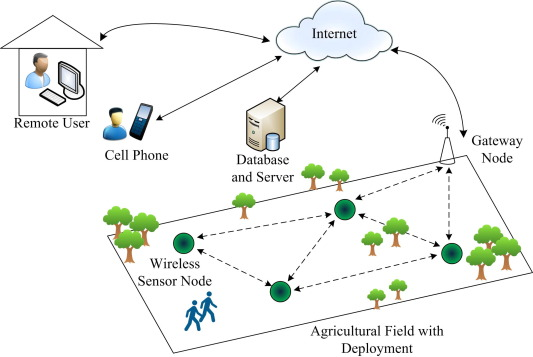
\includegraphics[width=0.75\textwidth]{fig1.jpg}
\caption{Wireless Sensor Network Deployment in Precision Agriculture Fields Showing Energy-Aware Clustering and Data Flow \cite{Musa2023}.}
\label{fig:wsn-ag}
\end{figure}

Another illustrative case involves livestock monitoring in pasturelands, where energy-aware protocols sustain wearable or collar-based sensors over extended grazing periods, transmitting health metrics via optimized multipath routes to central analytics hubs. These practical insights affirm that protocol selection must align with specific agronomic contexts, with empirical validations from field trials confirming the theoretical energy models' predictive accuracy in diverse climatic zones. Figure~\ref{fig:energy-patterns} visually contrasts cumulative energy dissipation, reinforcing the superiority of hybrid AI approaches in sustaining long-term precision farming operations.

\begin{figure}[htbp]
\centering
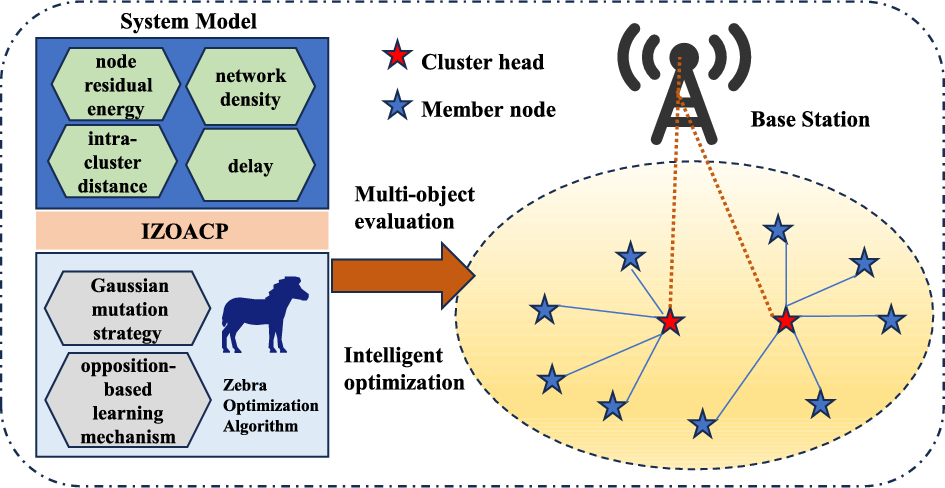
\includegraphics[width=0.75\textwidth]{fig2.jpg}
\caption{Energy Consumption Patterns Across Routing Protocols in Agricultural WSN Simulations \cite{Jawad2017}.}
\label{fig:energy-patterns}
\end{figure}

\begin{figure}[htbp]
\centering
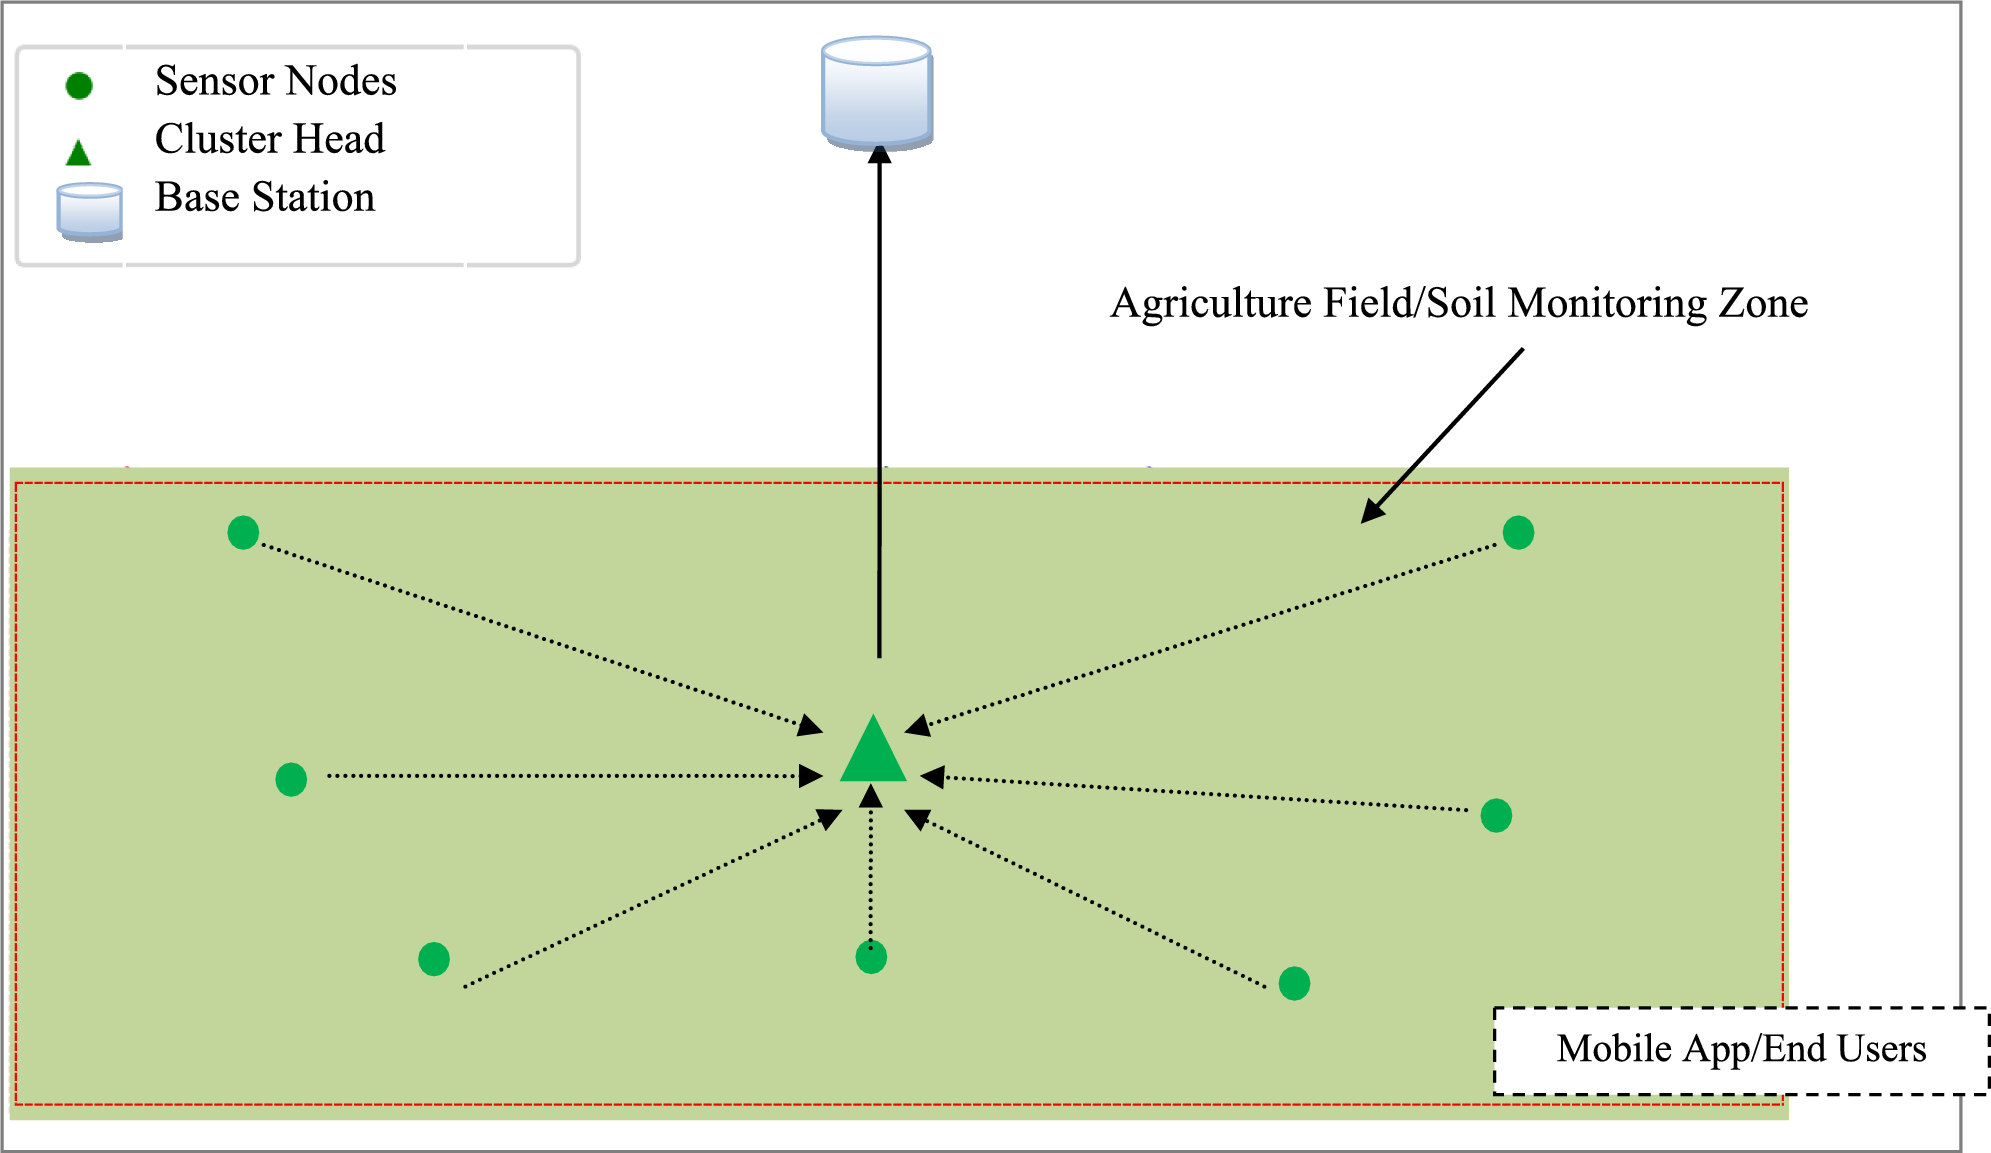
\includegraphics[width=0.75\textwidth]{fig3.jpg}
\caption{Diagram of the First-Order Radio Energy Model Applied to Wireless Sensor Networks in Smart Agriculture \cite{DelValleSoto2020}.}
\label{fig:energy-model}
\end{figure}

\subsection{Deployments in Arid Crop Systems}

Deployments in arid regions emphasize LEACH's clustering for water-scarce environments, where energy savings directly translate to extended irrigation decision cycles.

\subsection{Greenhouse and Controlled Environment Applications}

In controlled greenhouses, PEGASIS and TEEN hybrids deliver precise microclimate data with minimal energy overhead, supporting sustainable horticultural practices.

\subsection{Livestock and Pasture Management Use Cases}

Livestock monitoring leverages multipath AI routing to maintain connectivity across mobile herds, providing health insights without frequent battery interventions.

\subsection{Integrated Drone-Sensor Hybrid Systems}

Hybrid systems integrating drones with ground WSNs utilize adaptive protocols to optimize data relay, enhancing coverage in large-scale precision farming operations.

\section{Challenges and Open Issues}

Despite advancements, energy-aware routing in smart agriculture confronts several persistent challenges that hinder widespread adoption. Scalability remains a primary concern, as expanding networks to encompass thousands of nodes across heterogeneous terrains introduces complexities in maintaining energy balance and avoiding communication bottlenecks exacerbated by foliage attenuation or soil conductivity variations. These scalability issues are compounded in multi-crop farms where sensor requirements differ markedly between zones.

Security vulnerabilities pose another critical issue, with routing protocols susceptible to attacks that could falsify agricultural data or drain node batteries through denial-of-service tactics, necessitating lightweight yet robust authentication mechanisms integrated without inflating energy footprints. Environmental factors such as extreme weather further challenge protocol robustness, as signal degradation can force rerouting that accelerates energy depletion.

Interoperability with emerging IoT ecosystems further complicates deployments, as legacy sensors must coexist with 5G-enabled nodes while preserving energy-aware optimizations. Economic barriers, including initial deployment costs for AI-capable hardware, limit accessibility for smallholder farmers in developing regions. Open issues include the limited incorporation of energy harvesting sources, such as solar or kinetic from wind in open fields, into adaptive routing decisions, and the lack of standardized benchmarks for evaluating protocols under realistic agricultural mobility and interference models. Ethical considerations around data privacy in shared farming networks also emerge as open challenges requiring interdisciplinary solutions.

These challenges underscore the need for continued research to bridge theoretical efficacy with practical resilience in precision farming contexts, where failures in routing can have direct economic and food security implications.

\subsection{Technical Scalability and Interoperability Hurdles}

Technical hurdles in scaling networks involve managing increased control overhead while maintaining energy efficiency, particularly when integrating diverse sensor vendors in smart agriculture platforms.

\subsection{Environmental and Security Vulnerabilities}

Environmental vulnerabilities arise from weather-induced signal loss, while security threats demand energy-light cryptographic solutions to protect routing integrity without compromising battery life.

\subsection{Economic and Accessibility Barriers}

Economic barriers constrain adoption among small-scale farmers, highlighting the need for cost-effective protocol implementations that democratize precision farming benefits.

\subsection{Ethical and Standardization Gaps}

Ethical gaps in data ownership and the absence of global standards for energy-aware agricultural WSNs represent open issues that future research must address to ensure equitable and sustainable deployment.

\section{Future Directions}

Future directions in energy-aware routing for smart agriculture point toward deeper integration of artificial intelligence with edge computing paradigms, enabling on-node predictive analytics that preemptively reroute data based on forecasted energy states derived from machine learning models trained on multi-seasonal farm datasets. Hybrid protocols combining reinforcement learning with blockchain for secure, energy-efficient consensus in distributed decision-making represent a promising avenue, particularly for collaborative farming cooperatives sharing sensor infrastructure. These advancements will facilitate real-time optimization that accounts for microclimatic forecasts integrated directly into routing decisions.

Advancements in nanoscale sensors and quantum-inspired optimization algorithms may further refine energy models, incorporating stochastic elements reflective of real environmental stochasticity in precision agriculture. Emphasis on sustainability will drive protocols that prioritize carbon-aware routing aligned with global climate goals, while standardization efforts could facilitate plug-and-play deployments across diverse agritech platforms. Integration with next-generation communication technologies, such as 6G, promises ultra-low-power transmissions that could revolutionize energy profiles in expansive fields.

Exploration of bio-inspired algorithms mimicking ant colony or bee swarm behaviors for multipath optimization holds potential to enhance adaptability in dynamic crop canopies. Ultimately, these trajectories aim to realize self-sustaining, intelligent wireless sensor ecosystems that not only conserve energy but actively contribute to regenerative farming practices. Collaborative research involving agronomists, computer scientists, and policymakers will be essential to translate these directions into deployable solutions.

\subsection{Advancements in AI and Edge Computing Integration}

AI and edge computing will enable localized decision-making that reduces reliance on central sinks, further lowering energy demands in future smart agriculture networks.

\subsection{Sustainability and Energy Harvesting Innovations}

Sustainability-focused directions emphasize harvesting integration, allowing protocols to dynamically incorporate renewable sources into energy-aware routing calculations.

\subsection{Standardization and 6G Convergence}

Standardization initiatives combined with 6G technologies will support seamless, low-energy connectivity for precision farming on a global scale.

\subsection{Bio-Inspired and Regenerative Protocol Designs}

Bio-inspired designs will promote regenerative approaches that align routing efficiency with ecological restoration goals in sustainable agriculture.

\section{Conclusion}

In summary, energy-aware routing protocols constitute an indispensable pillar for the successful implementation of wireless sensor networks in smart agriculture and precision farming. Through detailed examination of foundational models, core hierarchical and AI-augmented approaches, comparative evaluations, practical deployments, challenges, and forward-looking strategies, this analysis affirms their capacity to extend network longevity, enhance data reliability, and support resource-efficient agricultural operations. The incorporation of precise energy consumption equations and empirical insights from field applications underscores the protocols' alignment with the multifaceted demands of modern farming.

As precision agriculture evolves toward greater automation and ecological integration, continued refinement of these routing mechanisms will be pivotal in unlocking full productivity gains while minimizing environmental footprints. This comprehensive framework provides a robust reference for researchers and practitioners seeking to advance sustainable agritech solutions through optimized wireless communications. Future efforts should focus on bridging remaining gaps to fully realize the potential of energy-aware systems in feeding a growing global population.

	\bibliographystyle{plain}
	\bibliography{references}
	
\end{document}